\chapter{Anwendung des Frameworks auf jadice flow}
\label{chap:anwendung}

In diesem Kapitel wird ein Architektur-Refactoring am Produkt \emph{jadice flow} geplant und in theoretischer Ebene durchgeführt.
Dazu wird das \gls{mmf} benutzt, das in \cref{sec:mmf} beschrieben wird.
Unterteilt ist der Prozess in drei Phasen, deren Durchführung im Folgenden beschrieben wird.

\section{Phase 1 - Architekturreview}

In dieser Phase wurde einer Fokusgruppe ein Architekturreview nach \Citet{SVAHNBERG20071893} wie in \cref{sec:methodik-architekturreview} beschrieben durchgeführt.
Teil dieser Gruppe waren vier Softwareentwickler beziehungsweise -Architekten
% Dabei handelt es sich um eine Architekturbewertungsmethode, die auf Szenarien-basierten Methoden wie \gls{saam} (\Citet{saam}) und \gls{atam} (\Citet{kazman_2000}) aufbaut.
% Stakeholder definieren gemeinsam gewünschte Szenarien und ordnen diesen \glspl{qa} zu.
% Außerdem wird den verschiedenen Szenarien jeweils ein Grad der Schwierigkeit und ein Grad der Wichtigkeit zugewiesen.
% Die resultierenden Szenarien können in den \gls{arh} eingegeben werden.

Die Szenarien, die sich dabei im konkreten Fall zu \emph{jadice flow} ergeben haben, sind in der \cref{tab:scenarios} zu sehen.

\begin{landscape}
	\begin{figure}
		\centering
		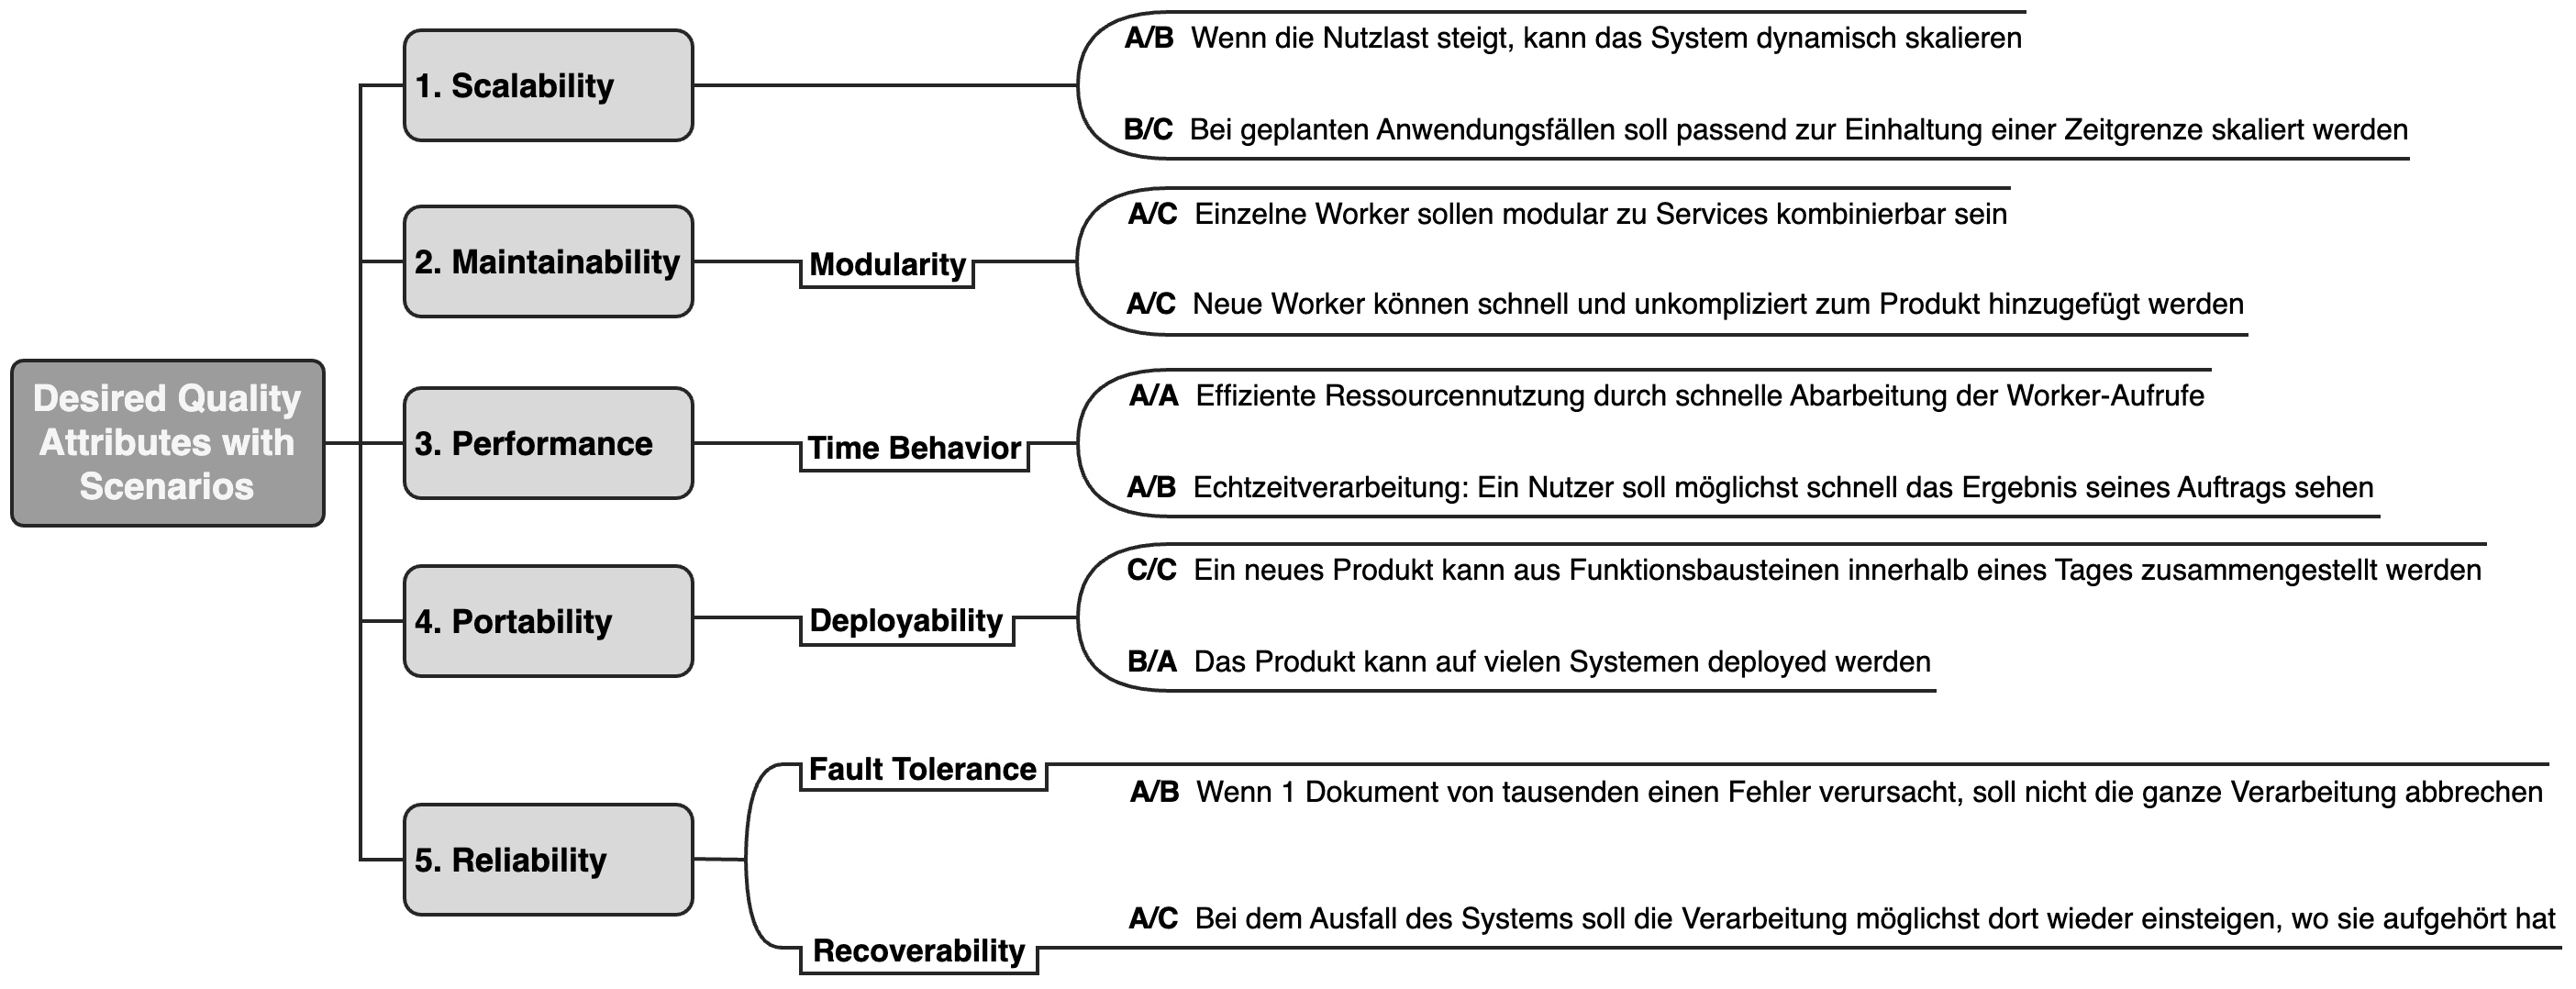
\includegraphics[width=1.5\textwidth]{scenarios.drawio}
		\caption[Utility Tree mit im Architekturreview ermittelten Qualitätsanforderungen und Szenarien]{
			Der Utility Tree mit Szenarien, die aus dem in Phase 1 durchgeführten Architekturreview resultieren.
			Von links nach rechts enthält der Baum folgende Elementarten: [1] Wurzel (ohne Bedeutung), [2] \gls{qa}, [3] Subattribut, [4] Beurteilung des Szenarios hinsichtlich Wichtigkeit und technischer Schwierigkeit, [5] Szenariobeschreibung.
		}
		\label{fig:scenarios}
	\end{figure}
\end{landscape}


\begin{table}
	\centering
	\begin{tabular}{ m{2,5cm} m{6cm} m{0.7cm} m{2,5cm} p{0.7cm} }
		\toprule
		\textbf{Name} & \textbf{Beschreibung} & \textbf{W/S} & \textbf{\glspl{qa}} & \textbf{MS} \\
		\midrule
		Dynamische Skalierbarkeit & Wenn die Nutzlast steigt, kann das System dynamisch skalieren & A/B & Scalability, Resource Utilization, Adaptability, Execution Cost & \advantage \\ \hline
		Statische Skalierbarkeit & Bei geplanten Anwendungsfällen soll passend zur Einhaltung einer Zeitgrenze skaliert werden & B/C & Scalability, Resource Utilization, Time Behavior & \advantage \\  \hline
		 Jobtemplates& Einzelne Worker sollen modular zu Services kombinierbar sein & A/C & Modularity, Reusability & - \\ \hline
		 Neue Worker& Neue Worker können schnell und unkompliziert zum Produkt hinzugefügt werden & A/C & Modularity, Reusability & \advantage  \\ \hline
		 Schnelle Abarbeitung & Effiziente Ressourcennutzung durch schnelle Abarbeitung der Worker-Aufrufe  & A/A & Time Behavior, Resource Utilization & \disadvantage \\ \hline
		 \glqq Echtzeit\grqq{}-Verarbeitung & Ein Nutzer soll möglichst schnell das Ergebnis seines Auftrags sehen & A/B & Time Behavior & \disadvantage \\ \hline
		 Einfaches Deployment & Ein neues Produkt kann aus Funktionsbausteinen innerhalb eines Tages zusammengestellt werden &C/C & Deployability, Modularity, Agility & \disadvantage \\ \hline
		 Platform-unabhängigkeit& Das Produkt kann auf vielen Systemen deployed werden & B/A & Deployability, Installability & \advantage \\ \hline
		 Fehlertoleranz Massen-verarbeitung & Wenn 1 Dokument von tausenden einen Fehler verursacht, soll nicht die ganze Verarbeitung abbrechen & A/B & Fault-Tolerance &\advantage \\ \hline
		 Erholen nach Systemausfall & Bei dem Ausfall des Systems soll die Verarbeitung möglichst dort wieder einsteigen, wo sie aufgehört hat & A/C & Recoverability & - \\
		\bottomrule
	\end{tabular}
	\caption[Im Architekturreview ermittelte Qualitätsanforderungen und Szenarien]{
		Szenarien, die aus dem in Phase 1 durchgeführten Architekturreview resultieren.
		\emph{W/S} gibt die Wichtigkeit/Schwierigkeit der Szenarien in drei Stufen an (A steht für sehr wichtig und sehr schwierig).
		\emph{\glspl{qa}} gibt die Assoziation der Szenarien zu bestimmten \acrfullpl{qa} an; zuerst genannte sind diejenigen, für die die Szenarien ursprünglich erstellt wurden.
		\emph{MS} gibt die Einschätzung darüber an, ob das jeweilige Szenario von einer Microservices-Architektur profitiert.
		}
	\label{tab:scenarios}
\end{table}

TODO nach Durchfürhung von Phase 1:
 - Beschreibung der Szenarien und QAs
 - Explizite Änderungsvorschläge


\section{Phase 2 - Strategieplanung}
\label{sec:durchführung-phase2}

\section{Phase 3a - Architekturplanung}
\section{Herausforderungen bei der Durchführung}
%\section{Analyse der Ergebnisse}
%\section{Erstellung eines Refactoring-Konzepts}
%\subsection{Bestimmung der optimalen Granularität}
%\subsection{Optimierung des Kommunikationsmodells und der Verringerung des IO-Flaschenhalses}
